\documentclass{beamer}
\usetheme{default} 

\setbeamercolor{structure}{fg=green!40!black} 
\usebackgroundtemplate{
    \centering
\includegraphics[width=\paperwidth,height=\paperheight]{images/android_wall}
}
\setbeamertemplate{navigation symbols}{}

\usepackage[polish]{babel}
\usepackage[utf8x]{inputenc}
\usepackage{t1enc}
\usepackage{default}
\usepackage{listings}

\lstset{language=java, basicstyle=\small, commentstyle=\color{gray}}
\lstset{frame=single}

\usefoottemplate{
  \vbox{
    \tinycolouredline{structure!25}{
      \color{black}\textbf{	
        \insertshortauthor\hfill
        Android @ Szczecin 2011
      } 
    }
%    \tinycolouredline{structure}{
%      \color{white}\textbf{\insertshorttitle}\hfill
%    } 
  }
}

\title{Android @ Szczecin \\ 2011}
\author{Konrad Malawski \\ konrad.malawski@java.pl}

\begin{document}




\begin{frame}
 \begin{center}
  \Huge{Moar* Fun with Views}
 \end{center}
\begin{flushright}
* sic
\end{flushright}
\end{frame}


\begin{frame}\frametitle{Zmierzamy w kierunku kolejnego Activity}
\begin{itemize}
 \item Dodamy nowe Activity
 \pause \item Będzie pobierać coś z sieci (lub udawać) oraz
 \pause \item hint: przyda się jakiś progress bar etc
 \pause \item utworzy z tych danych ListView
 \pause \item przejdziemy do niego przez \textbf{menu} w obecnym Activity
\end{itemize}
\end{frame}

% Menus
\begin{frame}
\begin{center}
 \Huge{Menu}
\end{center}
\end{frame}


\begin{frame}\frametitle{Menu (vide przycisk menu)}
\begin{center}
 Cel:\\
 \begin{figure}
  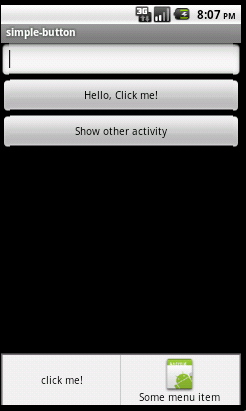
\includegraphics[height=.75\textheight]{images/sample_with_menu}
 \end{figure}
\end{center}
\end{frame}

\begin{frame}[fragile]\frametitle{res/menu/sample\_menu.xml}
\begin{lstlisting}
<menu xmlns:android="http://...">

    <item android:id="@+id/click_me_menu_item"
          android:title="click me!"
            />

    <item android:id="@+id/some_menu_item"
          android:title="Some menu item"
          android:icon="@drawable/icon"
            />
</menu>
\end{lstlisting}
\end{frame}

\begin{frame}[fragile]\frametitle{SomeActivity\#onCreateOptionsMenu}
\begin{lstlisting}
@Override
public boolean onCreateOptionsMenu(Menu menu) { 
  MenuInflater inflater = getMenuInflater();

  inflater.inflate(R.menu.sample_menu, menu);
  return true;
}
\end{lstlisting}
\end{frame}

\begin{frame}[fragile]\frametitle{SomeActivity\#onCreateOptionsMenu}
\begin{lstlisting}
@Override
public boolean onCreateOptionsMenu(Menu menu) { 
  MenuInflater inflater = getMenuInflater();

  inflater.inflate(R.menu.sample_menu, menu);
  return true; // true == ma zostac pokazane
}
\end{lstlisting}
\end{frame}

\begin{frame}[fragile]\frametitle{SomeActivity\#onOptionsItemSelected}
\begin{lstlisting}
@Override
public boolean onOptionsItemSelected(MenuItem item) {
  int itemId = item.getItemId();

  switch (itemId){
    case R.id.click_me_menu_item:
      doSomething();
      break;
    default:
      Log.i(TAG, "Some weird action was requested");
  }

  return true; 
}
\end{lstlisting}
\end{frame}

\begin{frame}[fragile]\frametitle{SomeActivity\#onOptionsItemSelected}
\begin{lstlisting}
@Override
public boolean onOptionsItemSelected(MenuItem item) {
  int itemId = item.getItemId();

  switch (itemId){
    case R.id.click_me_menu_item:
      doSomething();
      break;
    default:
      Log.i(TAG, "Some weird action was requested");
      return false;
  }

  return true; // true == obsluzylismy event
               //      == no need to bubble it
}
\end{lstlisting}
\end{frame}


% MORE FUN UI STUFF
\begin{frame}
\begin{center}
 \Huge{Giving Feedback} \\
 \large{(Toasts and Dialogs)}
\end{center}
\end{frame}


\begin{frame}[fragile]\frametitle{Pyszne tosty z masełkiem (android.widget.Toast)}

\begin{figure}[h]
 \centering
 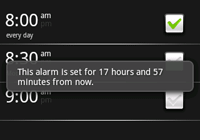
\includegraphics[height=0.40\textheight,keepaspectratio=true]{images/toast}
\end{figure}

 Przykład użycia: 
 \begin{lstlisting}
Toast.makeText(getApplicationContext(), // note: explain Context !
               "Halo Szczecin!", 
               Toast.LENGTH_LONG)
     .show();
 \end{lstlisting}

\end{frame}

\begin{frame}[fragile]
\frametitle{Co więcej potrafi Toast?}
\begin{lstlisting}
 Toast t = Toast.makeText(MyActivity.this, txt, LENGTH_SHORT);
\end{lstlisting}

\pause

Można mu zmienić pozycję:
\begin{lstlisting}
t.setGravity(Gravity.TOP|Gravity.LEFT, 0, 0);
\end{lstlisting}

\pause

lub podmienić widok:
\begin{lstlisting}
View customView = findViewById(R.id.custom_view);
/**/
t.setView(customView)
 \end{lstlisting}

\end{frame}

\begin{frame}
 \begin{center}
  \Huge{Dialog}
 \end{center}
\end{frame}


\begin{frame}\frametitle{Dialog - wyskakuje 'nad' Activity}
\begin{columns}
 \column{.5\textwidth}
  \begin{figure}
   \centering
   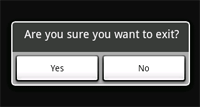
\includegraphics[width=.7\textwidth]{images/dialog_buttons}
  \end{figure}
  \begin{figure}
   \centering
   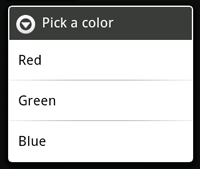
\includegraphics[width=.7\textwidth]{images/dialog_list}
  \end{figure}
 \column{.5\textwidth}
 \begin{figure}
   \centering
   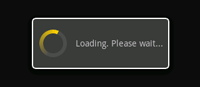
\includegraphics[width=.7\textwidth]{images/dialog_progress_spinning}
  \end{figure}
  \begin{figure}
   \centering
   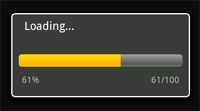
\includegraphics[width=.7\textwidth]{images/dialog_progress_bar}
  \end{figure}
\end{columns}
\end{frame}

% \begin{frame}[fragile]\frametitle{List Dialog}
% \begin{lstlisting}
% final CharSequence[] items = {"Red", "Green", "Blue"};
% 
% AlertDialog.Builder builder = new AlertDialog.Builder(this);
% builder.setTitle("Pick a color");
% builder.setItems(items, new DialogInterface.OnClickListener() {
%  public void onClick(DialogInterface dialog, int item) {
%   Toast.makeText(getApplicationContext(), items[item], Toast.LENGTH_SHORT).show();
%  }
% });
% AlertDialog alert = builder.create();
% \end{lstlisting}
% \end{frame}

\begin{frame}[fragile]\frametitle{Progress Dialog (Spinning)}
\begin{lstlisting}
ProgressDialog dialog = ProgressDialog
                           .show(MyActivity.this, 
                                 "", 
                                 "Loading. Please wait...", 
                                 true);
\end{lstlisting}

\begin{figure}
 \centering
 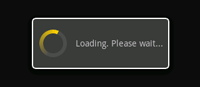
\includegraphics[width=.5\textwidth]{images/dialog_progress_spinning}
\end{figure}

\pause

\begin{lstlisting}
dialog.hide();
\end{lstlisting}
\end{frame}

\begin{frame}\frametitle{Slooooooooow stuff}
Dotychczas siedzieliśmy na tzw. ,,Main Thread''.
\begin{itemize}
 \item Zajmuje się on m.in. rysowaniem komponentów
 \item Jest współdzielony między Activity oraz Service!
 \item \textbf{,,Zajęcie'' głównego wątku na zbyt długo spowoduje UBICIE naszej aplikacji!}
\end{itemize}
\end{frame}

\begin{frame}[fragile]\frametitle{Slooooooooow stuff}
Introducing: \textbf{LazyWorker.java}:
\begin{lstlisting}
public class LazyWorker {
  List<String> getData() {
    sleep(10000); 

    return data;
  }
  
  void sleep(int howLong) { /**/ }
}
\end{lstlisting}
Będzie on udawał pobieranie danych z sieci.
\end{frame}

\begin{frame}[fragile]\frametitle{Fun Fact: \textbf{NetworkOnMainThreadException}}

Od wersji 3.0, Android \textbf{wymusza} korzystanie z wątków celem robienia czegokolwiek
związanego z siecią.\\ 
W przypadku zawołania np. \verb|GET(''http://google.com'');| na będąc na MainThread, 
zostanie rzucony wyjątek:

\begin{center}
  \textbf{android.os.NetworkOnMainThreadException}
 \end{center}

\begin{flushright}
\small{GET - fikcyjna implementacja pobierająca content z sieci}
\end{flushright}
\end{frame}

\begin{frame}\frametitle{Więc... new Thread()?}
\begin{center}
 ,,My się wątków nie boimy!''\\
 oświadczył dzielny rycerz.\\

\pause 
\ \\
\ \\
Szybko jednak zmienił zdanie, znajdywszy się w paszczy Mutexowego smoka.
\end{center}
\end{frame}

\begin{frame}
 \begin{center}
  \Huge{AsyncTask}
 \end{center}
\end{frame}

\begin{frame}
 \begin{center}
  \Huge{AsyncTask\\ <Params, Progress, Result>}
 \end{center}
\end{frame}


\begin{frame}[fragile]\frametitle{AsyncTask<Params, Progress, Result>}
Jedna z śliczniejszych abstrakcji na zadania asynchroniczne w API Androida.\\
\ \\
Podstawowa implementacja wygląda tak:

\begin{lstlisting}
new AsyncTask<Void, Void, Void>(){
  Void doInBackground(Void... voids){
    /**/
  }
}.execute();
\end{lstlisting}

\pause

Anyone remember \textbf{java.lang.Void}? :-)

\end{frame}


\begin{frame}[fragile]\frametitle{AsyncTask<Params, Progress, Result>}
Typowe zastosowanie, ,,pobieracz'' danych:
\begin{lstlisting}
List<String> datas = 
  new AsyncTask<Void, Integer, List<String>>() {
    @Override
    protected List<String> doInBackground(Void... voids) {
      return /* get stuff from the internet */;
    }
  }.execute() // not blocking
   .get(); // blocking
\end{lstlisting}
\end{frame}

\begin{frame}[fragile]\frametitle{AsyncTask<Params, Progress, Result>}
Typowe zastosowanie, ,,worker'' + ,,zestaw danych'':
\begin{lstlisting}
String[] data = getData();

new AsyncTask<String, Integer, Void>() {

  protected void onPreExecute(){
    Log.i(TAG, "Warning, will download the internet!")
  }

  protected List<String> doInBackground(Void... voids) {
    return /* get stuff from the internet */;
  }

  protected void onPreExecute(Void result) { // result
    Log.i(TAG, "Wow, we've downloaded the web!")
  }
}.execute(data); // varargs!
//.execute("a", "b", "c", "d"); // przypomnienie
\end{lstlisting}
\end{frame}

\begin{frame}[fragile]\frametitle{AsyncTask + ProgressDialog}
\begin{lstlisting}
final ProgressDialog d
             = new ProgressDialog(MyAct.this);
d.setProgressStyle(ProgressDialog.STYLE_HORIZONTAL);
d.setMessage("Loading details...");
d.setCancelable(false);
\end{lstlisting}
\end{frame}

%%%%%%%%%%%%%%%%%%%%%%%%%%%%%%%%%%%%%%%%%%%%%%%%%%%%%%%%%%%%%%%%%%%%%%%%%%%%%%%%%%%
%%%%%%%%%%%%%%%%%%%%%%%%%%%%%%%%%%%%%%%%%%%%%%%%%%%%%%%%%%%%%%%%%%%%%%%%%%%%%%%%%%%
%%%%%%%%%todo opisac HANDLER oraz jak AsyncTask moze publikowac progress %%%%%%%%%%
%%%%%%%%%%%%%%%%%%%%%%%%%%%%%%%%%%%%%%%%%%%%%%%%%%%%%%%%%%%%%%%%%%%%%%%%%%%%%%%%%%%
%%%%%%%%%%%%%%%%%%%%%%%%%%%%%%%%%%%%%%%%%%%%%%%%%%%%%%%%%%%%%%%%%%%%%%%%%%%%%%%%%%%

\begin{frame}[fragile]\frametitle{AsyncTask + ProgressDialog}
\begin{lstlisting}
Handler handler = new Handler();

final List<String> finalData = data;
progressDialog.setMax(data.size());

new AsyncTask<String, Integer, Void>() {
  @Override
  protected void onPreExecute() { /**/ }

  @Override
  protected void onPostExecute(Void aVoid) { /**/ }

  @Override
  protected Void doInBackground(String... strings) { /**/ }

  @Override
  protected void onProgressUpdate(Integer... values) { /**/ }
}.execute(data);
\end{lstlisting}
\end{frame}

\begin{frame}[fragile]\frametitle{AsyncTask + ProgressDialog}
Simple version: 
\begin{lstlisting}
@Override
protected void onPreExecute() {
  progressDialog.show();
}
\end{lstlisting}
\verb|progressDialog| musi być zadeklatowany final powyżej.
\end{frame}

\begin{frame}[fragile]\frametitle{AsyncTask + ProgressDialog}
Przy pomocy statycznego pomocnika:
\begin{lstlisting}

ProgressDialog dialog;

@Override
protected void onPreExecute() {
  this.dialog = ProgressDialog
                   .show(TasksActivity.this, 
                         "Loading", 
                         "Loading details...", 
                         true, 
                         false);
}
\end{lstlisting}
Unikamy zaśmiecania scope powyżej finalną zmienną.\\
Dałoby się również tutaj tradycyjnym \textbf{new} zrobić to samo.
\end{frame}

\begin{frame}[fragile]\frametitle{AsyncTask + ProgressDialog (\textbf{Overkill}, do not use)}
Sposób z handlerem, na wypadek źle zbindowanego ProgressDialog z którym musimy sobie jakoś poradzić. \\
Nie koniecznie w tej sytuacji dobre wyjście, ale to tylko przykład:
\begin{lstlisting}
@Override
protected void onPreExecute() {
  handler.post(new Runnable() {
    @Override
    public void run() {
      dialog.show();
    }
  });
}
\end{lstlisting}
Jest to o tyle ciekawe że \textbf{handler}owi możemy wysyłać na przykład tylko proste wiadomości zamiast Runnable etc.
\end{frame}


\begin{frame}[fragile]\frametitle{AsyncTask + ProgressDialog}
Jedyna z omawianych metod wołana w tle (nie na ,,UIThread'').
\begin{lstlisting}
@Override
protected Void doInBackground(String... strings) {
  int i = 1;
  for (final String data : finalDatas) {
    Details details = lazyWorker.getDetails(data);
    //...

    publishProgress(i++);
  }

  return null;
}
\end{lstlisting}
\end{frame}

\begin{frame}[fragile]\frametitle{AsyncTask + ProgressDialog}
Tutaj przydaje się handler, jeślibyśmy chcieli notyfikować co właśnie ,,opracowuje'' doInBackground.
\begin{lstlisting}
@Override
protected Void doInBackground(String... strings) {
  int i = 1;
  for (final String data : finalDatas) {
    final Details details = lazyWorker.getDetails(data);

    handler.post(new Runnable() {
      public void run() {
        Toast.makeText(TasksActivity.this, 
                       "processed: " + details, 
                       Toast.LENGTH_SHORT)
            .show();
      }
    });
    publishProgress(i++);
  }

  return null;
}
\end{lstlisting}
\end{frame}

\begin{frame}[fragile]\frametitle{AsyncTask + ProgressDialog}
,,Publikowanie postępów'':
\begin{lstlisting}
    doInBackground...  doInBackground...
       |   \               /  |
       |    publishProgress   | // async
       V                      V
  onProgressUpdate    onProgressUpdate
\end{lstlisting}
\end{frame}


\begin{frame}[fragile]\frametitle{AsyncTask + ProgressDialog}
Odbieranie informacji o postępach, ponownie wracamy na \textbf{UIThread} tutaj.
\begin{lstlisting}
@Override
protected void onProgressUpdate(Integer... values) {
  progressDialog.setProgress(values[0]);
}
\end{lstlisting}
\end{frame}

\begin{frame}[fragile]\frametitle{AsyncTask + ProgressDialog}
\begin{lstlisting}
@Override
protected void onPostExecute(Void aVoid) {
  progressDialog.dismiss();
}
\end{lstlisting}
Istnieje również \textbf{ProgressDialog\#hide()}, jednak w tym 
przypadku chcemy zwolnić również zasoby po tym dialogu.
\end{frame}








\end{document}
